% Asset ID: A21ParametricEquationsTikZ-002
% Source: Transcript section 1; CCEA A21-CG-LO001.
% Related lesson section: Worked Example 1; Common Mistakes and Exam Traps.
% Purpose: Show how -3<t<3 restricts y=x^2/4.

\documentclass[tikz,border=8pt]{standalone}
\usepackage{amsmath}
\usepackage{pgfplots}
\pgfplotsset{compat=1.18}
\begin{document}
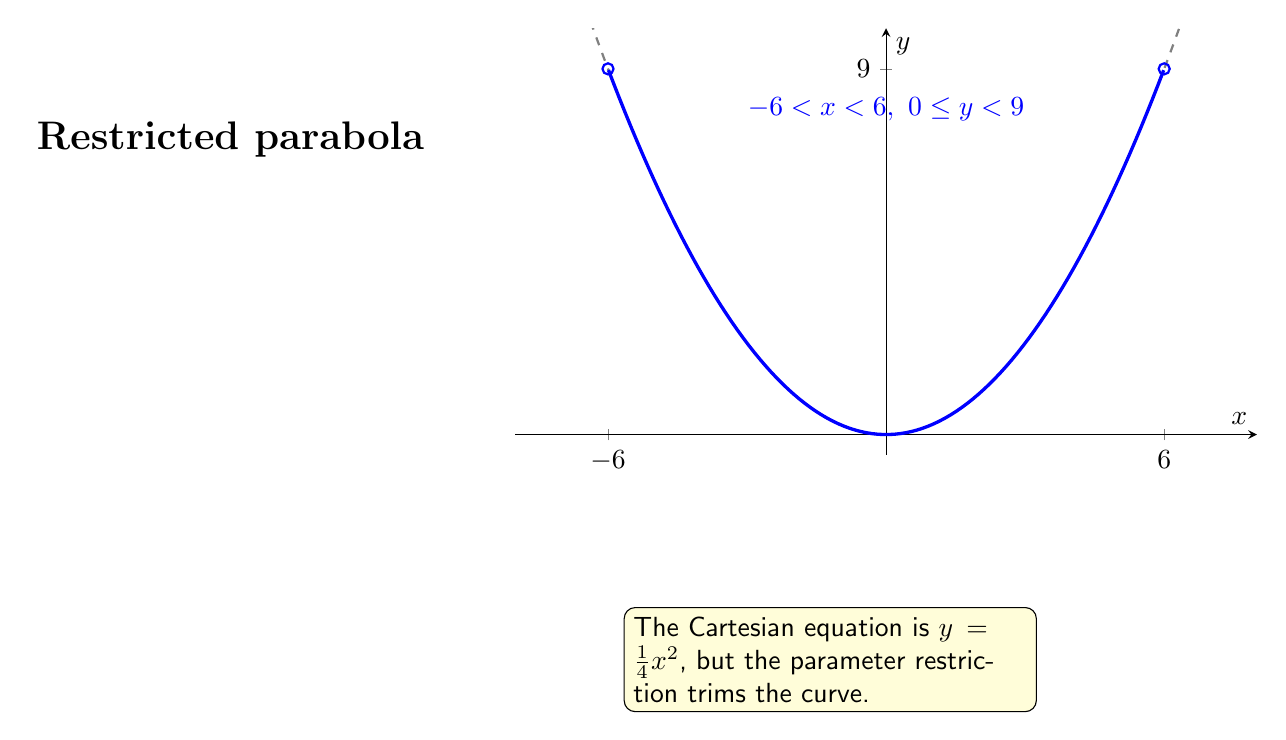
\begin{tikzpicture}[font=\sffamily]

\node[anchor=west, font=\bfseries\Large] at (-6.2,4.0) {Restricted parabola};
\begin{axis}[width=11cm,height=7cm,axis lines=middle,xmin=-8,xmax=8,ymin=-0.5,ymax=10,xtick={-6,0,6},ytick={0,9},xlabel={$x$},ylabel={$y$}]
\addplot[domain=-8:8,samples=100,gray,dashed,thick] {x^2/4};
\addplot[domain=-5.99:5.99,samples=100,blue,very thick] {x^2/4};
\addplot[only marks,mark=o,blue,thick] coordinates {(-6,9) (6,9)};
\node[blue] at (axis cs:0,8) {\(-6<x<6,\ 0\le y<9\)};
\end{axis}
\node[draw, rounded corners, fill=yellow!15, text width=5cm] at (4,-2.6) {The Cartesian equation is \(y=\frac14x^2\), but the parameter restriction trims the curve.};

\end{tikzpicture}
\end{document}
